% Options for packages loaded elsewhere
\PassOptionsToPackage{unicode}{hyperref}
\PassOptionsToPackage{hyphens}{url}
%
\documentclass[
]{article}
\usepackage{amsmath,amssymb}
\usepackage{iftex}
\ifPDFTeX
  \usepackage[T1]{fontenc}
  \usepackage[utf8]{inputenc}
  \usepackage{textcomp} % provide euro and other symbols
\else % if luatex or xetex
  \usepackage{unicode-math} % this also loads fontspec
  \defaultfontfeatures{Scale=MatchLowercase}
  \defaultfontfeatures[\rmfamily]{Ligatures=TeX,Scale=1}
\fi
\usepackage{lmodern}
\ifPDFTeX\else
  % xetex/luatex font selection
\fi
% Use upquote if available, for straight quotes in verbatim environments
\IfFileExists{upquote.sty}{\usepackage{upquote}}{}
\IfFileExists{microtype.sty}{% use microtype if available
  \usepackage[]{microtype}
  \UseMicrotypeSet[protrusion]{basicmath} % disable protrusion for tt fonts
}{}
\makeatletter
\@ifundefined{KOMAClassName}{% if non-KOMA class
  \IfFileExists{parskip.sty}{%
    \usepackage{parskip}
  }{% else
    \setlength{\parindent}{0pt}
    \setlength{\parskip}{6pt plus 2pt minus 1pt}}
}{% if KOMA class
  \KOMAoptions{parskip=half}}
\makeatother
\usepackage{xcolor}
\usepackage[margin=1in]{geometry}
\usepackage{color}
\usepackage{fancyvrb}
\newcommand{\VerbBar}{|}
\newcommand{\VERB}{\Verb[commandchars=\\\{\}]}
\DefineVerbatimEnvironment{Highlighting}{Verbatim}{commandchars=\\\{\}}
% Add ',fontsize=\small' for more characters per line
\usepackage{framed}
\definecolor{shadecolor}{RGB}{248,248,248}
\newenvironment{Shaded}{\begin{snugshade}}{\end{snugshade}}
\newcommand{\AlertTok}[1]{\textcolor[rgb]{0.94,0.16,0.16}{#1}}
\newcommand{\AnnotationTok}[1]{\textcolor[rgb]{0.56,0.35,0.01}{\textbf{\textit{#1}}}}
\newcommand{\AttributeTok}[1]{\textcolor[rgb]{0.13,0.29,0.53}{#1}}
\newcommand{\BaseNTok}[1]{\textcolor[rgb]{0.00,0.00,0.81}{#1}}
\newcommand{\BuiltInTok}[1]{#1}
\newcommand{\CharTok}[1]{\textcolor[rgb]{0.31,0.60,0.02}{#1}}
\newcommand{\CommentTok}[1]{\textcolor[rgb]{0.56,0.35,0.01}{\textit{#1}}}
\newcommand{\CommentVarTok}[1]{\textcolor[rgb]{0.56,0.35,0.01}{\textbf{\textit{#1}}}}
\newcommand{\ConstantTok}[1]{\textcolor[rgb]{0.56,0.35,0.01}{#1}}
\newcommand{\ControlFlowTok}[1]{\textcolor[rgb]{0.13,0.29,0.53}{\textbf{#1}}}
\newcommand{\DataTypeTok}[1]{\textcolor[rgb]{0.13,0.29,0.53}{#1}}
\newcommand{\DecValTok}[1]{\textcolor[rgb]{0.00,0.00,0.81}{#1}}
\newcommand{\DocumentationTok}[1]{\textcolor[rgb]{0.56,0.35,0.01}{\textbf{\textit{#1}}}}
\newcommand{\ErrorTok}[1]{\textcolor[rgb]{0.64,0.00,0.00}{\textbf{#1}}}
\newcommand{\ExtensionTok}[1]{#1}
\newcommand{\FloatTok}[1]{\textcolor[rgb]{0.00,0.00,0.81}{#1}}
\newcommand{\FunctionTok}[1]{\textcolor[rgb]{0.13,0.29,0.53}{\textbf{#1}}}
\newcommand{\ImportTok}[1]{#1}
\newcommand{\InformationTok}[1]{\textcolor[rgb]{0.56,0.35,0.01}{\textbf{\textit{#1}}}}
\newcommand{\KeywordTok}[1]{\textcolor[rgb]{0.13,0.29,0.53}{\textbf{#1}}}
\newcommand{\NormalTok}[1]{#1}
\newcommand{\OperatorTok}[1]{\textcolor[rgb]{0.81,0.36,0.00}{\textbf{#1}}}
\newcommand{\OtherTok}[1]{\textcolor[rgb]{0.56,0.35,0.01}{#1}}
\newcommand{\PreprocessorTok}[1]{\textcolor[rgb]{0.56,0.35,0.01}{\textit{#1}}}
\newcommand{\RegionMarkerTok}[1]{#1}
\newcommand{\SpecialCharTok}[1]{\textcolor[rgb]{0.81,0.36,0.00}{\textbf{#1}}}
\newcommand{\SpecialStringTok}[1]{\textcolor[rgb]{0.31,0.60,0.02}{#1}}
\newcommand{\StringTok}[1]{\textcolor[rgb]{0.31,0.60,0.02}{#1}}
\newcommand{\VariableTok}[1]{\textcolor[rgb]{0.00,0.00,0.00}{#1}}
\newcommand{\VerbatimStringTok}[1]{\textcolor[rgb]{0.31,0.60,0.02}{#1}}
\newcommand{\WarningTok}[1]{\textcolor[rgb]{0.56,0.35,0.01}{\textbf{\textit{#1}}}}
\usepackage{graphicx}
\makeatletter
\def\maxwidth{\ifdim\Gin@nat@width>\linewidth\linewidth\else\Gin@nat@width\fi}
\def\maxheight{\ifdim\Gin@nat@height>\textheight\textheight\else\Gin@nat@height\fi}
\makeatother
% Scale images if necessary, so that they will not overflow the page
% margins by default, and it is still possible to overwrite the defaults
% using explicit options in \includegraphics[width, height, ...]{}
\setkeys{Gin}{width=\maxwidth,height=\maxheight,keepaspectratio}
% Set default figure placement to htbp
\makeatletter
\def\fps@figure{htbp}
\makeatother
\setlength{\emergencystretch}{3em} % prevent overfull lines
\providecommand{\tightlist}{%
  \setlength{\itemsep}{0pt}\setlength{\parskip}{0pt}}
\setcounter{secnumdepth}{-\maxdimen} % remove section numbering
\ifLuaTeX
  \usepackage{selnolig}  % disable illegal ligatures
\fi
\IfFileExists{bookmark.sty}{\usepackage{bookmark}}{\usepackage{hyperref}}
\IfFileExists{xurl.sty}{\usepackage{xurl}}{} % add URL line breaks if available
\urlstyle{same}
\hypersetup{
  pdftitle={BIO00066I Cell Biology: Workshop 2},
  hidelinks,
  pdfcreator={LaTeX via pandoc}}

\title{BIO00066I Cell Biology: Workshop 2}
\author{}
\date{\vspace{-2.5em}2023-12-17}

\begin{document}
\maketitle

{
\setcounter{tocdepth}{2}
\tableofcontents
}
\hypertarget{step-0-make-a-r-studio-project.}{%
\section{Step 0: Make a R Studio
project.}\label{step-0-make-a-r-studio-project.}}

There are two ways to do this:

\begin{enumerate}
\def\labelenumi{\arabic{enumi}.}
\tightlist
\item
  Open the \textbf{File} menu, and choose \textbf{New Project}.
\item
  Use the Projects drop-down menu at the very \textbf{top right} of the
  R Studio window
\end{enumerate}

\begin{center}\rule{0.5\linewidth}{0.5pt}\end{center}

\hypertarget{setting-up-the-r-studio-environment}{%
\subsection{Setting up the R Studio
environment}\label{setting-up-the-r-studio-environment}}

First, we set up our R Studio environment, with these commands:

\begin{Shaded}
\begin{Highlighting}[]
\CommentTok{\#clear previous data}
\FunctionTok{rm}\NormalTok{(}\AttributeTok{list=}\FunctionTok{ls}\NormalTok{())}

\CommentTok{\#The tidyverse!}
\FunctionTok{library}\NormalTok{(tidyverse)}
\end{Highlighting}
\end{Shaded}

\begin{verbatim}
## -- Attaching core tidyverse packages ------------------------ tidyverse 2.0.0 --
## v dplyr     1.1.3     v readr     2.1.4
## v forcats   1.0.0     v stringr   1.5.0
## v ggplot2   3.4.3     v tibble    3.2.1
## v lubridate 1.9.3     v tidyr     1.3.0
## v purrr     1.0.2     
## -- Conflicts ------------------------------------------ tidyverse_conflicts() --
## x dplyr::filter() masks stats::filter()
## x dplyr::lag()    masks stats::lag()
## i Use the conflicted package (<http://conflicted.r-lib.org/>) to force all conflicts to become errors
\end{verbatim}

\begin{Shaded}
\begin{Highlighting}[]
\CommentTok{\#we need this to make pretty plots with the \textquotesingle{}ggarrange\textquotesingle{} package}
\FunctionTok{library}\NormalTok{(ggpubr)}
\end{Highlighting}
\end{Shaded}

\begin{center}\rule{0.5\linewidth}{0.5pt}\end{center}

\hypertarget{getting-to-know-the-data}{%
\subsection{Getting to know the data}\label{getting-to-know-the-data}}

Load the data and see what it looks like.

We will load some data from a website.

\begin{Shaded}
\begin{Highlighting}[]
\NormalTok{cells}\OtherTok{\textless{}{-}}\FunctionTok{read\_tsv}\NormalTok{(}\FunctionTok{url}\NormalTok{(}\StringTok{"https://djeffares.github.io/data/BIO00066I/A1{-}FFT.tsv"}\NormalTok{))}
\end{Highlighting}
\end{Shaded}

\begin{verbatim}
## Rows: 21291 Columns: 23
## -- Column specification --------------------------------------------------------
## Delimiter: "\t"
## dbl (23): frame, untracked, tracking.id, lineage.id, position.x.um, position...
## 
## i Use `spec()` to retrieve the full column specification for this data.
## i Specify the column types or set `show_col_types = FALSE` to quiet this message.
\end{verbatim}

\hypertarget{first-glimpses-of-the-data}{%
\subsubsection{First glimpses of the
data}\label{first-glimpses-of-the-data}}

The \textbf{cells} object is a \emph{tibble}, which is a tidyverse
version of a \emph{data frame}, with rows (which are usually different
observations) and columns (which are usually different features or
aspects of the observations). Like an excel spreadsheet.

It is important to know what data you have in your tibble. I like to
know:

\begin{itemize}
\tightlist
\item
  How many rows and columns there are
\item
  What the column names are
\item
  What types of values the columns of data have (numeric, factors, or
  text?)
\end{itemize}

Here are some ways to find this out for our \textbf{cells} tibble.

\begin{enumerate}
\def\labelenumi{\arabic{enumi}.}
\tightlist
\item
  Use the \textbf{view(cells)} command (shows the data in a popup
  window)
\item
  Use the \textbf{glimpse(cells)} command (counts rows and columns, and
  shows some of the data)
\item
  Use the \textbf{summary(cells)} command (shows a summary of averages,
  medians and so on)
\end{enumerate}

Try \textbf{view} now. This will open a new tab that looks like excel.

You can close this tab, or just clock back you your script.

\begin{Shaded}
\begin{Highlighting}[]
\CommentTok{\#try view}
\FunctionTok{view}\NormalTok{(cells)}
\end{Highlighting}
\end{Shaded}

Now try glimpse

\begin{Shaded}
\begin{Highlighting}[]
\FunctionTok{glimpse}\NormalTok{(cells)}
\end{Highlighting}
\end{Shaded}

\begin{verbatim}
## Rows: 21,291
## Columns: 23
## $ frame                             <dbl> 1, 2, 1, 3, 4, 5, 6, 7, 8, 9, 10, 11~
## $ untracked                         <dbl> 1, 1, 1, 1, 1, 1, 1, 1, 1, 1, 1, 1, ~
## $ tracking.id                       <dbl> 1, 1, 2, 2, 2, 2, 2, 2, 2, 2, 2, 2, ~
## $ lineage.id                        <dbl> 1, 1, 2, 2, 2, 2, 2, 2, 2, 2, 2, 2, ~
## $ position.x.um                     <dbl> 33.22, 22.37, 123.18, 132.67, 135.97~
## $ position.y.um                     <dbl> 1323.33, 1333.63, 1025.47, 1020.06, ~
## $ pixel.position.x.pixels           <dbl> 49, 33, 185, 199, 204, 205, 201, 194~
## $ pixel.position.y.pixels           <dbl> 1989, 2004, 1541, 1533, 1538, 1547, ~
## $ volume.um                         <dbl> 1206.85, 1102.60, 1554.09, 1705.12, ~
## $ mean.thickness.um                 <dbl> 1.2483838, 1.3124160, 1.0051419, 1.0~
## $ radius.um                         <dbl> 17.54194, 16.35303, 22.18449, 22.584~
## $ area.um                           <dbl> 966.73, 840.13, 1546.14, 1602.36, 15~
## $ sphericity                        <dbl> 0.273, 0.297, 0.205, 0.208, 0.203, 0~
## $ length.um                         <dbl> 74.21, 48.61, 60.44, 120.85, 121.43,~
## $ width.um                          <dbl> 23.69, 24.44, 46.80, 33.34, 40.18, 4~
## $ orientation                       <dbl> -70.55, -65.55, 34.50, 26.72, 27.47,~
## $ dry.mass.pg                       <dbl> 301.71, 275.65, 388.52, 426.28, 398.~
## $ displacement.um                   <dbl> 0.00, 14.96, 0.00, 10.92, 12.93, 14.~
## $ instantaneous.velocity.um.per.s   <dbl> 0.000000000, 0.010829316, 0.00000000~
## $ instantaneous.velocity.x.um.per.s <dbl> 0.00000, -0.00785, 0.00000, 0.00344,~
## $ instantaneous.velocity.y.um.per.s <dbl> 0.00000, 0.00746, 0.00000, -0.00195,~
## $ track.length.um                   <dbl> 0.00, 14.96, 0.00, 10.92, 15.74, 21.~
## $ perimeter.um                      <dbl> 174.97, 127.07, 186.95, 251.48, 270.~
\end{verbatim}

We have 21291 rows, and 23 columns. The \textbf{glimpse} command shows
information about each column on a new line like:

\textbf{\#\# \$ frame 1, 2, 1}

We have column names like: \emph{frame}, \emph{untracked} and
\emph{tracking.id}.

The \textbf{} on each line means that the data type is a numeric values
with decimal points.

It is important to use at least one of these when you first read in a
new data set - to check that it is all OK.

\begin{center}\rule{0.5\linewidth}{0.5pt}\end{center}

\hypertarget{saving-data-ans-scripts-data-hygiene}{%
\subsubsection{Saving data ans scripts: data
hygiene}\label{saving-data-ans-scripts-data-hygiene}}

It is important to save your work regularly, and to be organised.
Organising files, data and scripts is called \textbf{data hygiene}. So
take these steps now to keep up your data hygiene:

\begin{itemize}
\tightlist
\item
  save your script (from the file menu, or the hot keys: ⌘S on a mac,
  ctrl-s on a PC)
\item
  save all your data objects using the \textbf{save.image} command as
  below
\end{itemize}

\begin{Shaded}
\begin{Highlighting}[]
\FunctionTok{save.image}\NormalTok{(}\StringTok{\textquotesingle{}BIO00066I.workshop2.2023{-}12{-}25.Rda\textquotesingle{}}\NormalTok{)}
\end{Highlighting}
\end{Shaded}

Why did I put \textbf{2023-12-25} in the file name?

This is a kind of \emph{date stamp} (it refers to Christmas day). Naming
files in this say helps you to keep track of when you made the file.
It's an element of data hygiene.

\begin{center}\rule{0.5\linewidth}{0.5pt}\end{center}

\hypertarget{making-plots}{%
\subsection{Making plots}\label{making-plots}}

From our first views of the data, it looks like we have these values
that could be important to understand.

\begin{itemize}
\tightlist
\item
  volume.um
\item
  radius.um
\item
  width.um
\item
  dry.mass.pgs
\item
  area.um
\item
  length.um
\end{itemize}

A good way of understanding data is to plot it.

PS: In all these values \textbf{um} means microns. These are usually
represented as \textbf{µm}.

\hypertarget{plot-a-histogram}{%
\subsubsection{Plot a histogram}\label{plot-a-histogram}}

Histograms can sometimes be useful.Let's see:

\begin{Shaded}
\begin{Highlighting}[]
\FunctionTok{ggplot}\NormalTok{(cells, }\FunctionTok{aes}\NormalTok{(}\AttributeTok{x=}\NormalTok{volume.um))}\SpecialCharTok{+}
  \FunctionTok{geom\_histogram}\NormalTok{()}
\end{Highlighting}
\end{Shaded}

\begin{verbatim}
## `stat_bin()` using `bins = 30`. Pick better value with `binwidth`.
\end{verbatim}

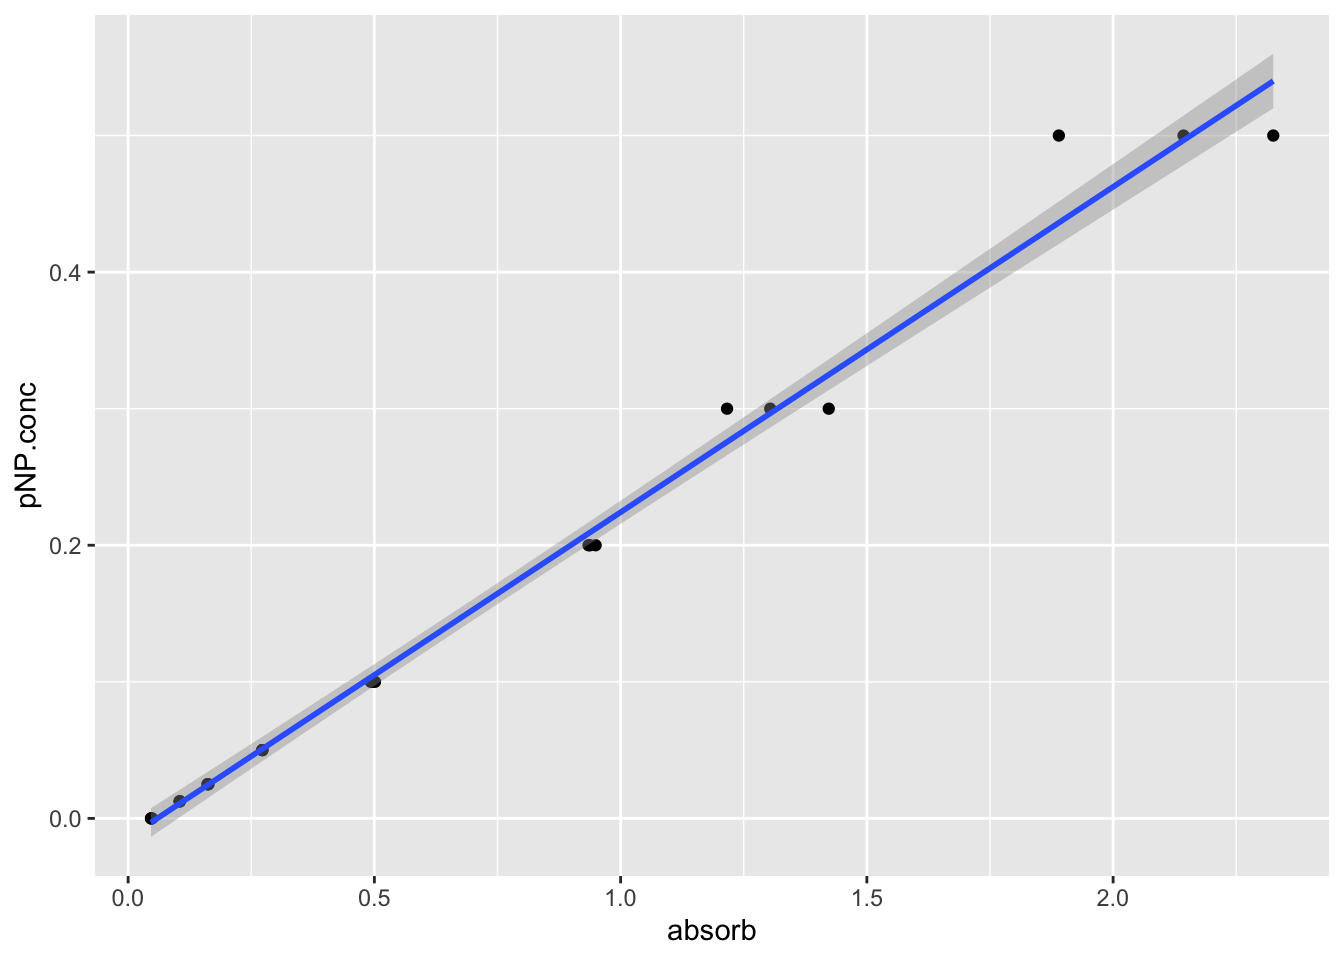
\includegraphics{BIO00066I-workshop2_files/figure-latex/unnamed-chunk-6-1.pdf}

\hypertarget{density-plots}{%
\subsubsection{Density plots}\label{density-plots}}

A density plot might be be better. So let's try that.

\begin{Shaded}
\begin{Highlighting}[]
\FunctionTok{ggplot}\NormalTok{(cells, }\FunctionTok{aes}\NormalTok{(}\AttributeTok{x=}\NormalTok{volume.um))}\SpecialCharTok{+}
  \FunctionTok{geom\_density}\NormalTok{()}\SpecialCharTok{+}
  \FunctionTok{theme\_light}\NormalTok{()}
\end{Highlighting}
\end{Shaded}

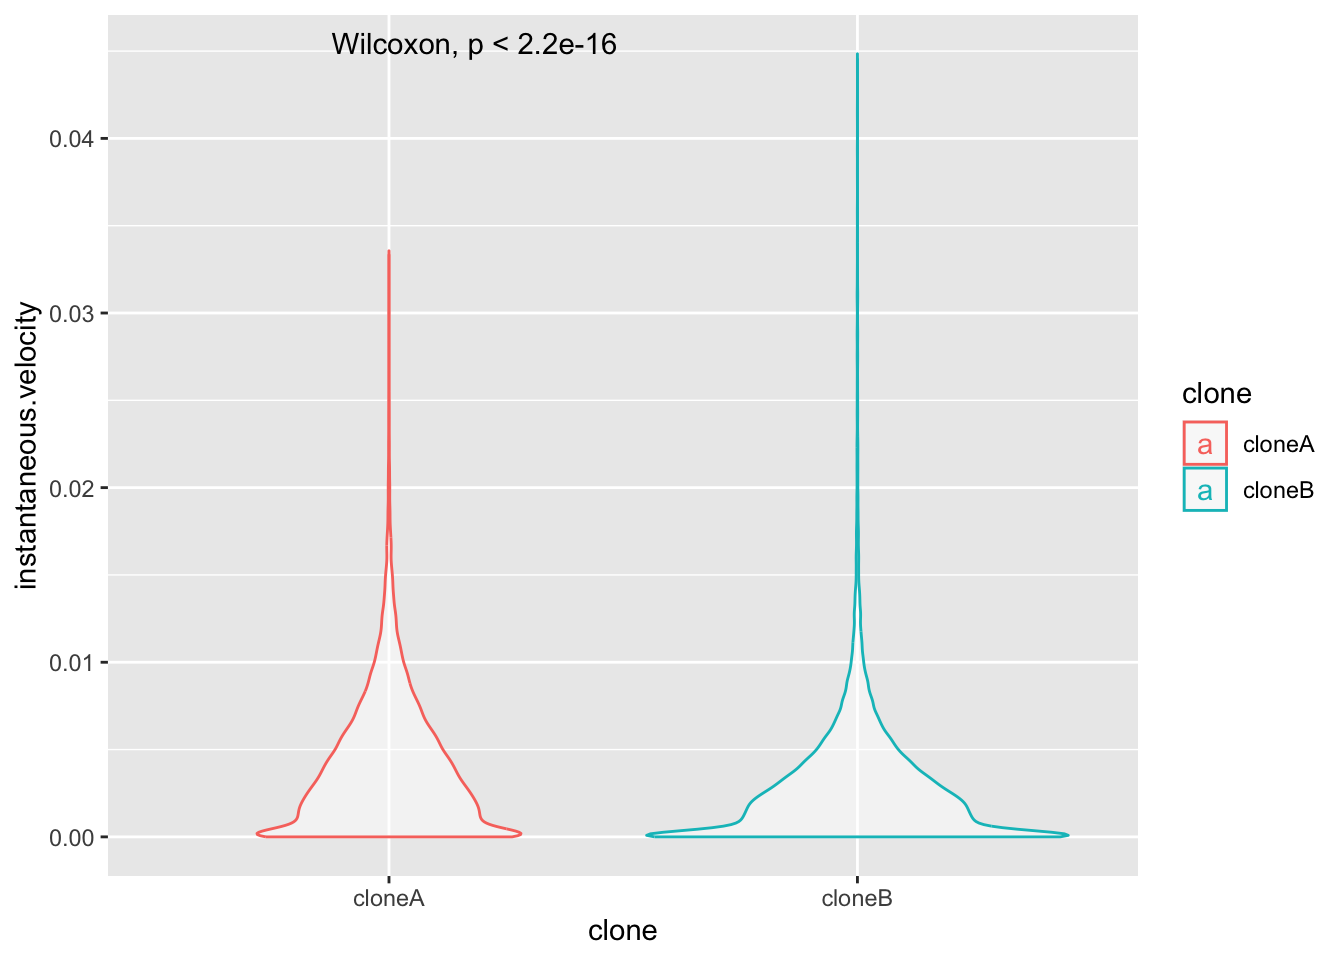
\includegraphics{BIO00066I-workshop2_files/figure-latex/unnamed-chunk-7-1.pdf}

Now examine the \textbf{radius} using a \textbf{density plot}.

\begin{Shaded}
\begin{Highlighting}[]
\FunctionTok{ggplot}\NormalTok{(cells, }\FunctionTok{aes}\NormalTok{(}\AttributeTok{x=}\NormalTok{radius.um))}\SpecialCharTok{+}
  \FunctionTok{geom\_density}\NormalTok{()}\SpecialCharTok{+}
  \FunctionTok{theme\_light}\NormalTok{()}
\end{Highlighting}
\end{Shaded}

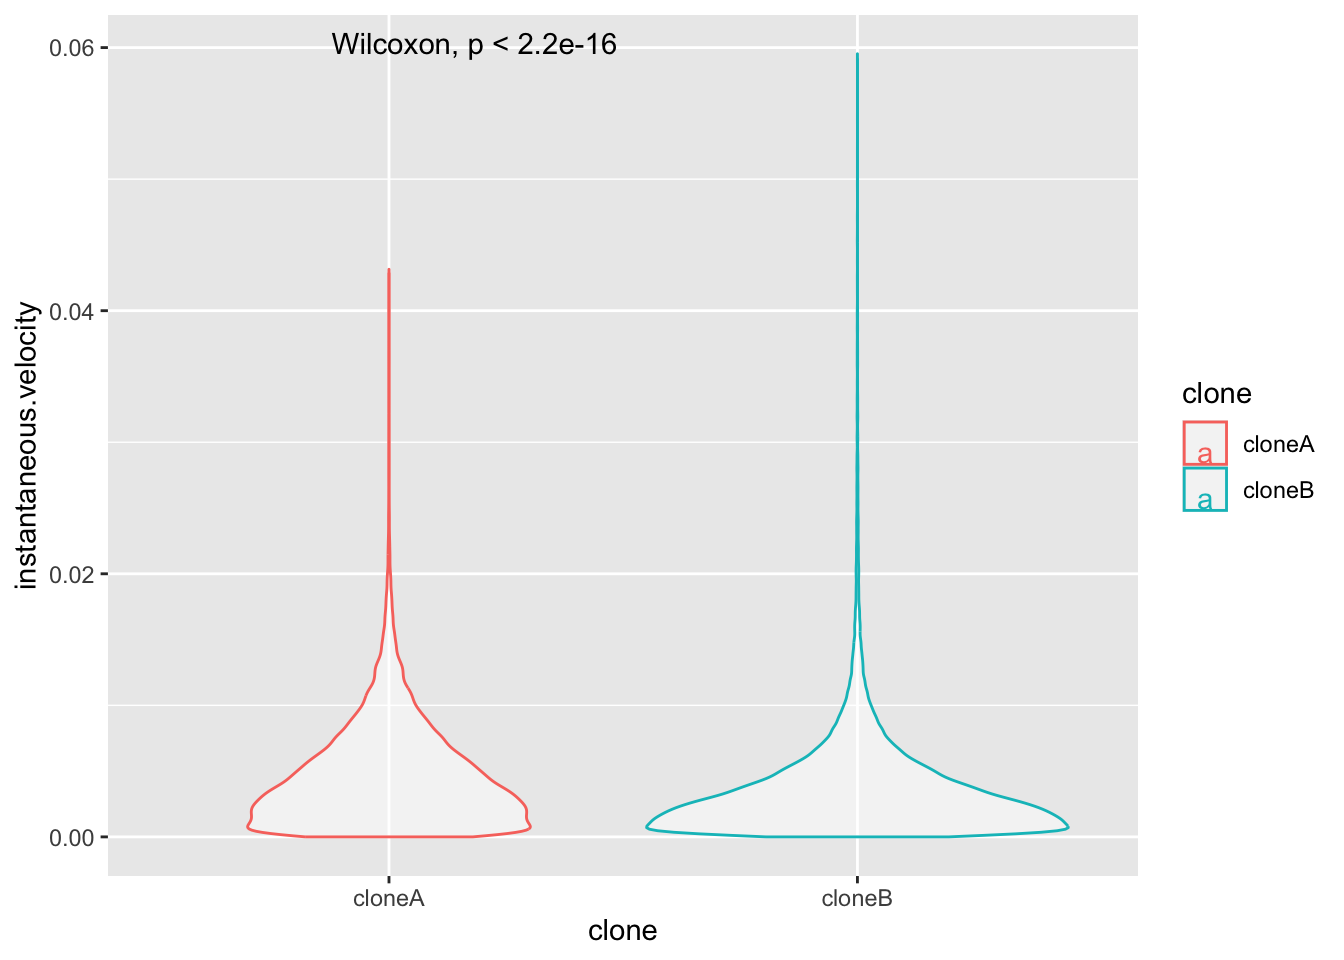
\includegraphics{BIO00066I-workshop2_files/figure-latex/unnamed-chunk-8-1.pdf}

Looks like there might be \textbf{two populations} here, perhaps?

\begin{center}\rule{0.5\linewidth}{0.5pt}\end{center}

\hypertarget{arranging-many-plots-together}{%
\subsubsection{Arranging many plots
together}\label{arranging-many-plots-together}}

Plot all the values now, \textbf{arrange} them and then \textbf{save} a
plot as a jpeg.

\begin{Shaded}
\begin{Highlighting}[]
\CommentTok{\#volumne}
\NormalTok{volume.plot}\OtherTok{\textless{}{-}}\FunctionTok{ggplot}\NormalTok{(cells, }\FunctionTok{aes}\NormalTok{(}\AttributeTok{x=}\NormalTok{width.um))}\SpecialCharTok{+}
  \FunctionTok{geom\_density}\NormalTok{()}\SpecialCharTok{+}
  \FunctionTok{theme\_light}\NormalTok{()}

\CommentTok{\#radius}
\NormalTok{radius.plot}\OtherTok{\textless{}{-}}\FunctionTok{ggplot}\NormalTok{(cells, }\FunctionTok{aes}\NormalTok{(}\AttributeTok{x=}\NormalTok{radius.um))}\SpecialCharTok{+}
  \FunctionTok{geom\_density}\NormalTok{()}\SpecialCharTok{+}
  \FunctionTok{theme\_light}\NormalTok{()}

\CommentTok{\#width}
\NormalTok{width.plot}\OtherTok{\textless{}{-}}\FunctionTok{ggplot}\NormalTok{(cells, }\FunctionTok{aes}\NormalTok{(}\AttributeTok{x=}\NormalTok{width.um))}\SpecialCharTok{+}
  \FunctionTok{geom\_density}\NormalTok{()}\SpecialCharTok{+}
  \FunctionTok{theme\_light}\NormalTok{()}

\CommentTok{\#dry.mass.pgs}
\NormalTok{mass.plot}\OtherTok{\textless{}{-}}\FunctionTok{ggplot}\NormalTok{(cells, }\FunctionTok{aes}\NormalTok{(}\AttributeTok{x=}\NormalTok{dry.mass.pg))}\SpecialCharTok{+}
  \FunctionTok{geom\_density}\NormalTok{()}\SpecialCharTok{+}
  \FunctionTok{theme\_light}\NormalTok{()}

\CommentTok{\#area.um}
\NormalTok{area.plot}\OtherTok{\textless{}{-}}\FunctionTok{ggplot}\NormalTok{(cells, }\FunctionTok{aes}\NormalTok{(}\AttributeTok{x=}\NormalTok{area.um))}\SpecialCharTok{+}
  \FunctionTok{geom\_density}\NormalTok{()}\SpecialCharTok{+}
  \FunctionTok{theme\_light}\NormalTok{()}

\CommentTok{\#length.um}
\NormalTok{length.plot}\OtherTok{\textless{}{-}}\FunctionTok{ggplot}\NormalTok{(cells, }\FunctionTok{aes}\NormalTok{(}\AttributeTok{x=}\NormalTok{length.um))}\SpecialCharTok{+}
  \FunctionTok{geom\_density}\NormalTok{()}\SpecialCharTok{+}
  \FunctionTok{theme\_light}\NormalTok{()}

\CommentTok{\#arrange the plot}
\NormalTok{density.plots}\OtherTok{\textless{}{-}}\FunctionTok{ggarrange}\NormalTok{(}
\NormalTok{  volume.plot,}
\NormalTok{  radius.plot,}
\NormalTok{  width.plot, }
\NormalTok{  mass.plot, }
\NormalTok{  area.plot,}
\NormalTok{  length.plot,}
  \AttributeTok{ncol =} \DecValTok{3}\NormalTok{, }
  \AttributeTok{nrow =} \DecValTok{2}
\NormalTok{)}

\CommentTok{\#now save a jpeg}
\CommentTok{\#the default width and height = 7}
\CommentTok{\#so lets make it a bit wider}
\FunctionTok{ggsave}\NormalTok{(density.plots,}
  \AttributeTok{file=}\StringTok{"plots/first.density.plots.jpeg"}\NormalTok{,}
  \AttributeTok{width =} \DecValTok{7}\SpecialCharTok{*}\FloatTok{1.5}\NormalTok{,}
  \AttributeTok{height =} \DecValTok{7}
\NormalTok{)}
\end{Highlighting}
\end{Shaded}

\begin{center}\rule{0.5\linewidth}{0.5pt}\end{center}

\hypertarget{reading-in-multiple-files}{%
\subsection{Reading in multiple files}\label{reading-in-multiple-files}}

So far we have looked at the data from one file: \textbf{A1-FFT.tsv}.
This contains XXX.

There is other data that is either replicate XXX, or a different cell
type (XXX).

The data we have are:

\textbf{three replicates of XXX} files:

\begin{itemize}
\tightlist
\item
  A1-FFT.tsv
\item
  A2-FFT.tsv\\
\item
  A3-FFT.tsv
\end{itemize}

\textbf{three replicates of XXX} files:

\begin{itemize}
\tightlist
\item
  B1-FFT.tsv
\item
  B2-FFT.tsv\\
\item
  B3-FFT.tsv
\end{itemize}

\begin{center}\rule{0.5\linewidth}{0.5pt}\end{center}

\hypertarget{reading-in-more-data-files}{%
\subsubsection{Reading in more data
files}\label{reading-in-more-data-files}}

First, read in the files on by one:

\begin{Shaded}
\begin{Highlighting}[]
\CommentTok{\#all the XXX files}
\NormalTok{A1 }\OtherTok{\textless{}{-}}\FunctionTok{read\_tsv}\NormalTok{(}\FunctionTok{url}\NormalTok{(}\StringTok{"https://djeffares.github.io/data/BIO00066I/A1{-}FFT.tsv"}\NormalTok{))}
\end{Highlighting}
\end{Shaded}

\begin{verbatim}
## Rows: 21291 Columns: 23
## -- Column specification --------------------------------------------------------
## Delimiter: "\t"
## dbl (23): frame, untracked, tracking.id, lineage.id, position.x.um, position...
## 
## i Use `spec()` to retrieve the full column specification for this data.
## i Specify the column types or set `show_col_types = FALSE` to quiet this message.
\end{verbatim}

\begin{Shaded}
\begin{Highlighting}[]
\NormalTok{A2 }\OtherTok{\textless{}{-}}\FunctionTok{read\_tsv}\NormalTok{(}\FunctionTok{url}\NormalTok{(}\StringTok{"https://djeffares.github.io/data/BIO00066I/A2{-}FFT.tsv"}\NormalTok{))}
\end{Highlighting}
\end{Shaded}

\begin{verbatim}
## Rows: 19948 Columns: 23
## -- Column specification --------------------------------------------------------
## Delimiter: "\t"
## dbl (22): frame, untracked, tracking.id, lineage.id, position.x.um, position...
## lgl  (1): perimeter.um
## 
## i Use `spec()` to retrieve the full column specification for this data.
## i Specify the column types or set `show_col_types = FALSE` to quiet this message.
\end{verbatim}

\begin{Shaded}
\begin{Highlighting}[]
\NormalTok{A3 }\OtherTok{\textless{}{-}}\FunctionTok{read\_tsv}\NormalTok{(}\FunctionTok{url}\NormalTok{(}\StringTok{"https://djeffares.github.io/data/BIO00066I/A3{-}FFT.tsv"}\NormalTok{))}
\end{Highlighting}
\end{Shaded}

\begin{verbatim}
## Rows: 14333 Columns: 23
## -- Column specification --------------------------------------------------------
## Delimiter: "\t"
## dbl (23): frame, untracked, tracking.id, lineage.id, position.x.um, position...
## 
## i Use `spec()` to retrieve the full column specification for this data.
## i Specify the column types or set `show_col_types = FALSE` to quiet this message.
\end{verbatim}

\begin{Shaded}
\begin{Highlighting}[]
\CommentTok{\#all the XXX files}
\NormalTok{B1 }\OtherTok{\textless{}{-}}\FunctionTok{read\_tsv}\NormalTok{(}\FunctionTok{url}\NormalTok{(}\StringTok{"https://djeffares.github.io/data/BIO00066I/B1{-}FFT.tsv"}\NormalTok{))}
\end{Highlighting}
\end{Shaded}

\begin{verbatim}
## Rows: 9100 Columns: 23
## -- Column specification --------------------------------------------------------
## Delimiter: "\t"
## dbl (23): frame, untracked, tracking.id, lineage.id, position.x.um, position...
## 
## i Use `spec()` to retrieve the full column specification for this data.
## i Specify the column types or set `show_col_types = FALSE` to quiet this message.
\end{verbatim}

\begin{Shaded}
\begin{Highlighting}[]
\NormalTok{B2 }\OtherTok{\textless{}{-}}\FunctionTok{read\_tsv}\NormalTok{(}\FunctionTok{url}\NormalTok{(}\StringTok{"https://djeffares.github.io/data/BIO00066I/B2{-}FFT.tsv"}\NormalTok{))}
\end{Highlighting}
\end{Shaded}

\begin{verbatim}
## Rows: 16445 Columns: 23
## -- Column specification --------------------------------------------------------
## Delimiter: "\t"
## dbl (23): frame, untracked, tracking.id, lineage.id, position.x.um, position...
## 
## i Use `spec()` to retrieve the full column specification for this data.
## i Specify the column types or set `show_col_types = FALSE` to quiet this message.
\end{verbatim}

\begin{Shaded}
\begin{Highlighting}[]
\NormalTok{B3 }\OtherTok{\textless{}{-}}\FunctionTok{read\_tsv}\NormalTok{(}\FunctionTok{url}\NormalTok{(}\StringTok{"https://djeffares.github.io/data/BIO00066I/B3{-}FFT.tsv"}\NormalTok{))}
\end{Highlighting}
\end{Shaded}

\begin{verbatim}
## Rows: 10796 Columns: 23
## -- Column specification --------------------------------------------------------
## Delimiter: "\t"
## dbl (23): frame, untracked, tracking.id, lineage.id, position.x.um, position...
## 
## i Use `spec()` to retrieve the full column specification for this data.
## i Specify the column types or set `show_col_types = FALSE` to quiet this message.
\end{verbatim}

Let's save our data again:

\begin{Shaded}
\begin{Highlighting}[]
\FunctionTok{save.image}\NormalTok{(}\StringTok{\textquotesingle{}BIO00066I.workshop2.2023{-}12{-}25.Rda\textquotesingle{}}\NormalTok{)}
\end{Highlighting}
\end{Shaded}

\begin{center}\rule{0.5\linewidth}{0.5pt}\end{center}

\hypertarget{using-bind_rows}{%
\subsubsection{Using bind\_rows}\label{using-bind_rows}}

Now we have many tibbles: cells, A1, A2, A3, B1, B2 and B3.

While its OK to have all these objects, many of the functions of
\href{https://www.tidyverse.org/}{the tidyverse}, are designed to work
with **one tibble* that contains all the data.

Let's put all the \textbf{A} data (XXX) into one tibble.

\begin{Shaded}
\begin{Highlighting}[]
\NormalTok{A.all}\OtherTok{\textless{}{-}}\FunctionTok{bind\_rows}\NormalTok{(}\FunctionTok{list}\NormalTok{(A1, A2, A3), }\AttributeTok{.id =} \StringTok{"replicate"}\NormalTok{)}
\end{Highlighting}
\end{Shaded}

Because we used \textbf{.id = ``replicate''} we should now have a new
column called \textbf{replicate}. Check it is present with:

\begin{Shaded}
\begin{Highlighting}[]
\FunctionTok{unique}\NormalTok{(A.all}\SpecialCharTok{$}\NormalTok{replicate)}
\end{Highlighting}
\end{Shaded}

Now put all the \textbf{B} data (YYY) into one tibble.

\begin{Shaded}
\begin{Highlighting}[]
\NormalTok{B.all}\OtherTok{\textless{}{-}}\FunctionTok{bind\_rows}\NormalTok{(}\FunctionTok{list}\NormalTok{(B1, B2, B3), }\AttributeTok{.id =} \StringTok{"replicate"}\NormalTok{)}
\end{Highlighting}
\end{Shaded}

\begin{center}\rule{0.5\linewidth}{0.5pt}\end{center}

\hypertarget{making-one-tidy-file}{%
\subsubsection{Making one tidy file}\label{making-one-tidy-file}}

We can use \textbf{bind\_rows} to bind A.all and B.all.

This time, it would be better to define the cell type XXX in a new
column, so we can identify this later. So let's add these now. It is
easy to add a new column to a tibble with, like this:

\begin{Shaded}
\begin{Highlighting}[]
\NormalTok{A.all}\SpecialCharTok{$}\NormalTok{cell.type}\OtherTok{=}\StringTok{\textquotesingle{}XXX\textquotesingle{}}
\NormalTok{B.all}\SpecialCharTok{$}\NormalTok{cell.type}\OtherTok{=}\StringTok{\textquotesingle{}YYY\textquotesingle{}}
\end{Highlighting}
\end{Shaded}

Finally do the bind\_rows:

\begin{Shaded}
\begin{Highlighting}[]
\NormalTok{cells}\OtherTok{\textless{}{-}}\FunctionTok{bind\_rows}\NormalTok{(A.all, B.all)}
\end{Highlighting}
\end{Shaded}

And do some careful checking, to examine what we have:

\begin{Shaded}
\begin{Highlighting}[]
\CommentTok{\#get a glimpse of the data:}
\FunctionTok{glimpse}\NormalTok{(cells)}
\end{Highlighting}
\end{Shaded}

\begin{verbatim}
## Rows: 91,913
## Columns: 25
## $ replicate                         <chr> "1", "1", "1", "1", "1", "1", "1", "~
## $ frame                             <dbl> 1, 2, 1, 3, 4, 5, 6, 7, 8, 9, 10, 11~
## $ untracked                         <dbl> 1, 1, 1, 1, 1, 1, 1, 1, 1, 1, 1, 1, ~
## $ tracking.id                       <dbl> 1, 1, 2, 2, 2, 2, 2, 2, 2, 2, 2, 2, ~
## $ lineage.id                        <dbl> 1, 1, 2, 2, 2, 2, 2, 2, 2, 2, 2, 2, ~
## $ position.x.um                     <dbl> 33.22, 22.37, 123.18, 132.67, 135.97~
## $ position.y.um                     <dbl> 1323.33, 1333.63, 1025.47, 1020.06, ~
## $ pixel.position.x.pixels           <dbl> 49, 33, 185, 199, 204, 205, 201, 194~
## $ pixel.position.y.pixels           <dbl> 1989, 2004, 1541, 1533, 1538, 1547, ~
## $ volume.um                         <dbl> 1206.85, 1102.60, 1554.09, 1705.12, ~
## $ mean.thickness.um                 <dbl> 1.2483838, 1.3124160, 1.0051419, 1.0~
## $ radius.um                         <dbl> 17.54194, 16.35303, 22.18449, 22.584~
## $ area.um                           <dbl> 966.73, 840.13, 1546.14, 1602.36, 15~
## $ sphericity                        <dbl> 0.273, 0.297, 0.205, 0.208, 0.203, 0~
## $ length.um                         <dbl> 74.21, 48.61, 60.44, 120.85, 121.43,~
## $ width.um                          <dbl> 23.69, 24.44, 46.80, 33.34, 40.18, 4~
## $ orientation                       <dbl> -70.55, -65.55, 34.50, 26.72, 27.47,~
## $ dry.mass.pg                       <dbl> 301.71, 275.65, 388.52, 426.28, 398.~
## $ displacement.um                   <dbl> 0.00, 14.96, 0.00, 10.92, 12.93, 14.~
## $ instantaneous.velocity.um.per.s   <dbl> 0.000000000, 0.010829316, 0.00000000~
## $ instantaneous.velocity.x.um.per.s <dbl> 0.00000, -0.00785, 0.00000, 0.00344,~
## $ instantaneous.velocity.y.um.per.s <dbl> 0.00000, 0.00746, 0.00000, -0.00195,~
## $ track.length.um                   <dbl> 0.00, 14.96, 0.00, 10.92, 15.74, 21.~
## $ perimeter.um                      <dbl> 174.97, 127.07, 186.95, 251.48, 270.~
## $ cell.type                         <chr> "XXX", "XXX", "XXX", "XXX", "XXX", "~
\end{verbatim}

\begin{Shaded}
\begin{Highlighting}[]
\CommentTok{\#check our column names}
\FunctionTok{names}\NormalTok{(cells)}
\end{Highlighting}
\end{Shaded}

\begin{verbatim}
##  [1] "replicate"                         "frame"                            
##  [3] "untracked"                         "tracking.id"                      
##  [5] "lineage.id"                        "position.x.um"                    
##  [7] "position.y.um"                     "pixel.position.x.pixels"          
##  [9] "pixel.position.y.pixels"           "volume.um"                        
## [11] "mean.thickness.um"                 "radius.um"                        
## [13] "area.um"                           "sphericity"                       
## [15] "length.um"                         "width.um"                         
## [17] "orientation"                       "dry.mass.pg"                      
## [19] "displacement.um"                   "instantaneous.velocity.um.per.s"  
## [21] "instantaneous.velocity.x.um.per.s" "instantaneous.velocity.y.um.per.s"
## [23] "track.length.um"                   "perimeter.um"                     
## [25] "cell.type"
\end{verbatim}

\hypertarget{save-your-data}{%
\subsubsection{Save your data!}\label{save-your-data}}

To finish up, we'll remove the A1, A2 \emph{etc}, and save our data
again.

Also - don't forget to save your script.

\begin{Shaded}
\begin{Highlighting}[]
\FunctionTok{rm}\NormalTok{(A1,A2,A3,B1,B2,B3)}
\FunctionTok{save.image}\NormalTok{(}\StringTok{\textquotesingle{}BIO00066I.workshop2.2023{-}12{-}25.Rda\textquotesingle{}}\NormalTok{)}
\end{Highlighting}
\end{Shaded}

\hypertarget{final-comments}{%
\subsection{Final comments}\label{final-comments}}

We now have a simple, saved tidyverse-compliant data file. We saved our
data in a file called \textbf{BIO00066I.workshop2.2023-12-25.Rda}.

\textbf{Keep this file somewhere safe, or email it to yourself.}

PS: It may feel like we didn't do very much biology today. But because
we created a simple tidy object all our data analysis will be much
easier from now on.

\hypertarget{end}{%
\subsection{End}\label{end}}

\end{document}
